%
% Another appendix chapter
\chapter{Towards Application}

% Challenges
\section{Challenges}
\subsection{Angular Momentum and Height Variation}
\begin{figure}[h]
  \begin{subfigure}{0.3\textwidth}
  \centering
  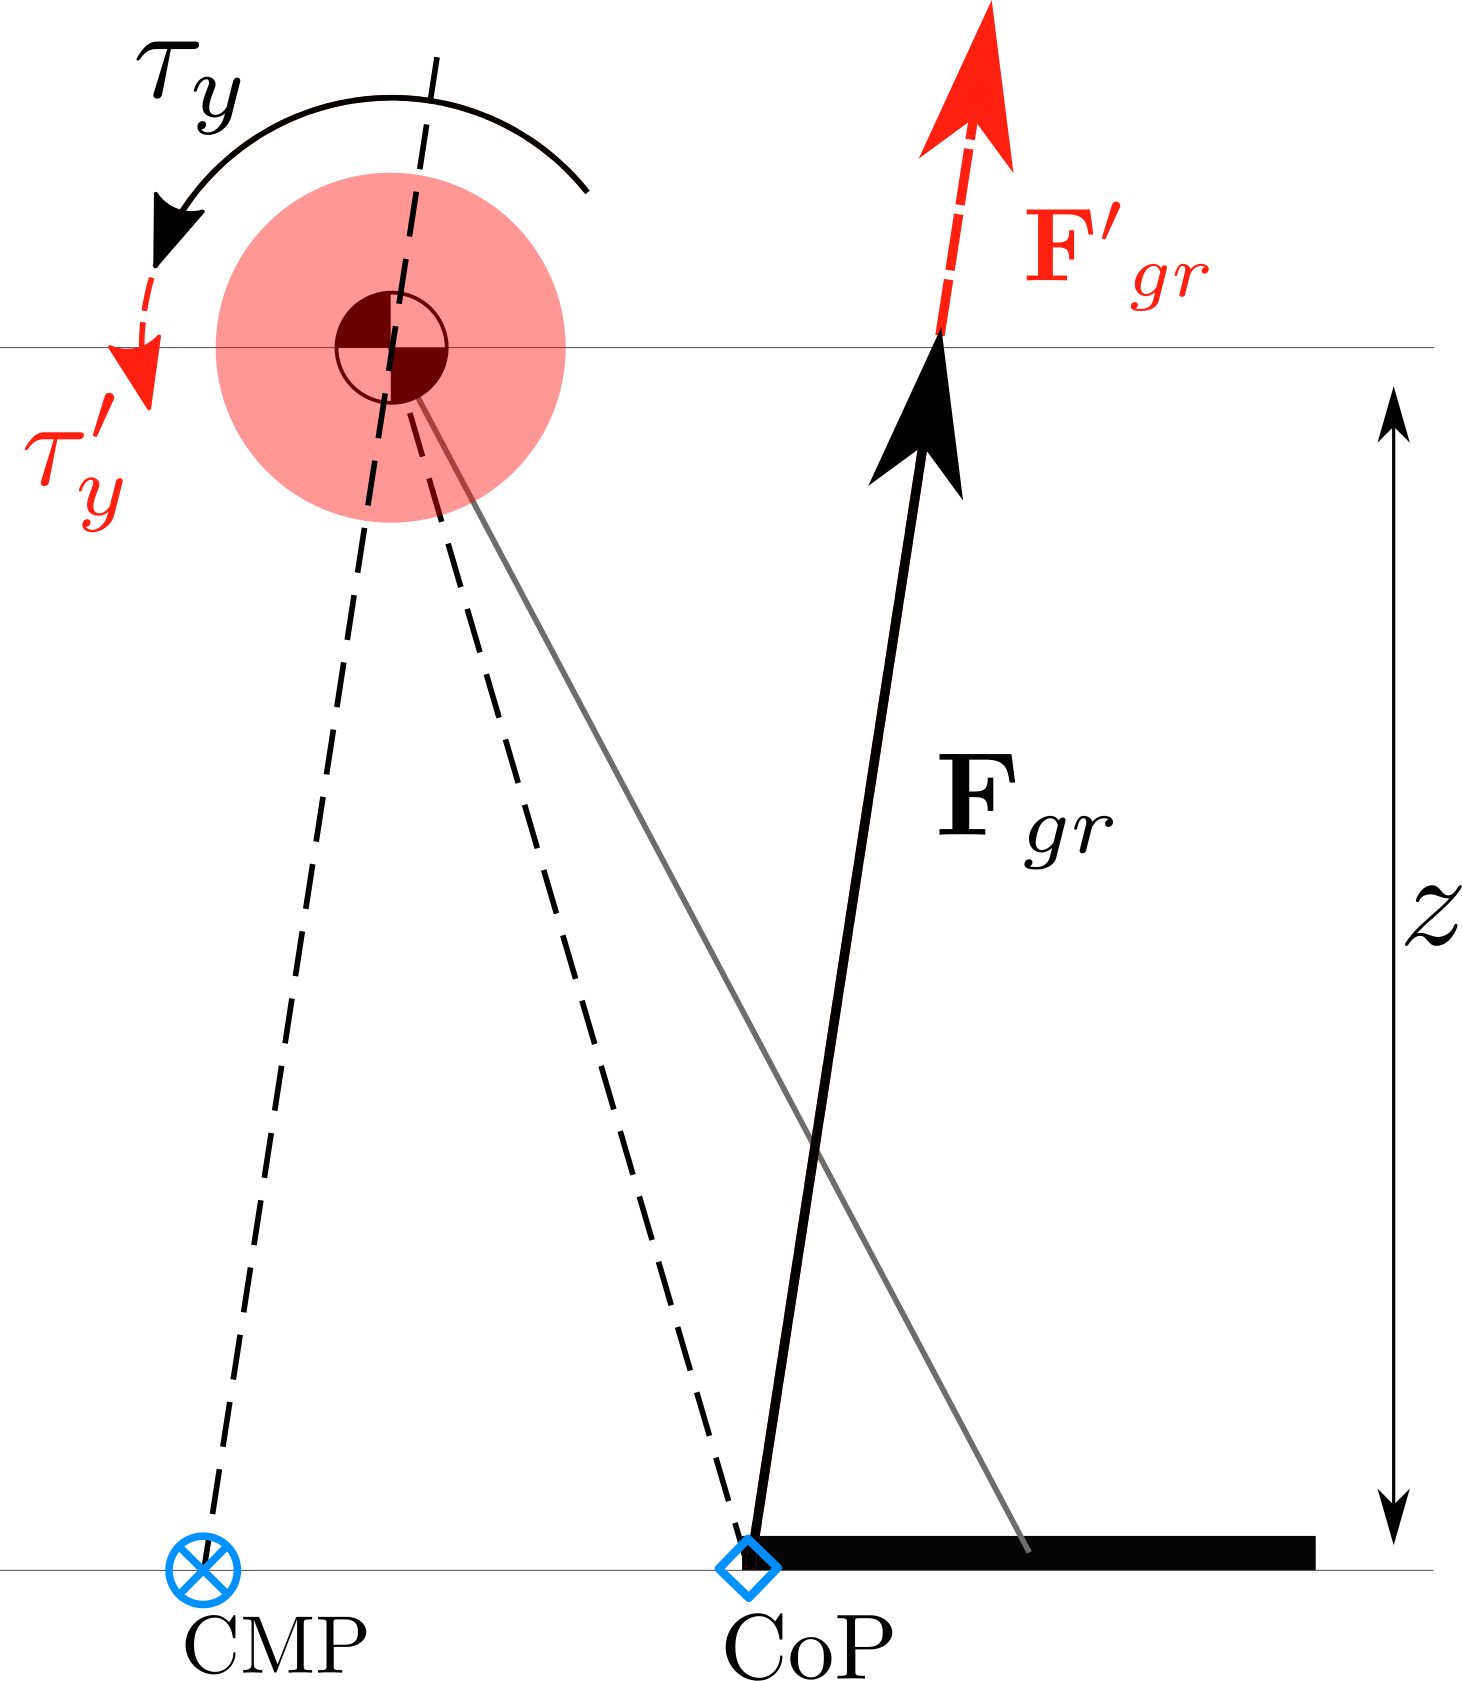
\includegraphics[width=.8\linewidth]{STYLESTUFF/2DCMPVIZ.png}
   \caption{}
    \label{fig:cmpFza}
  \end{subfigure}
  \begin{subfigure}{0.3\textwidth}
    \centering
  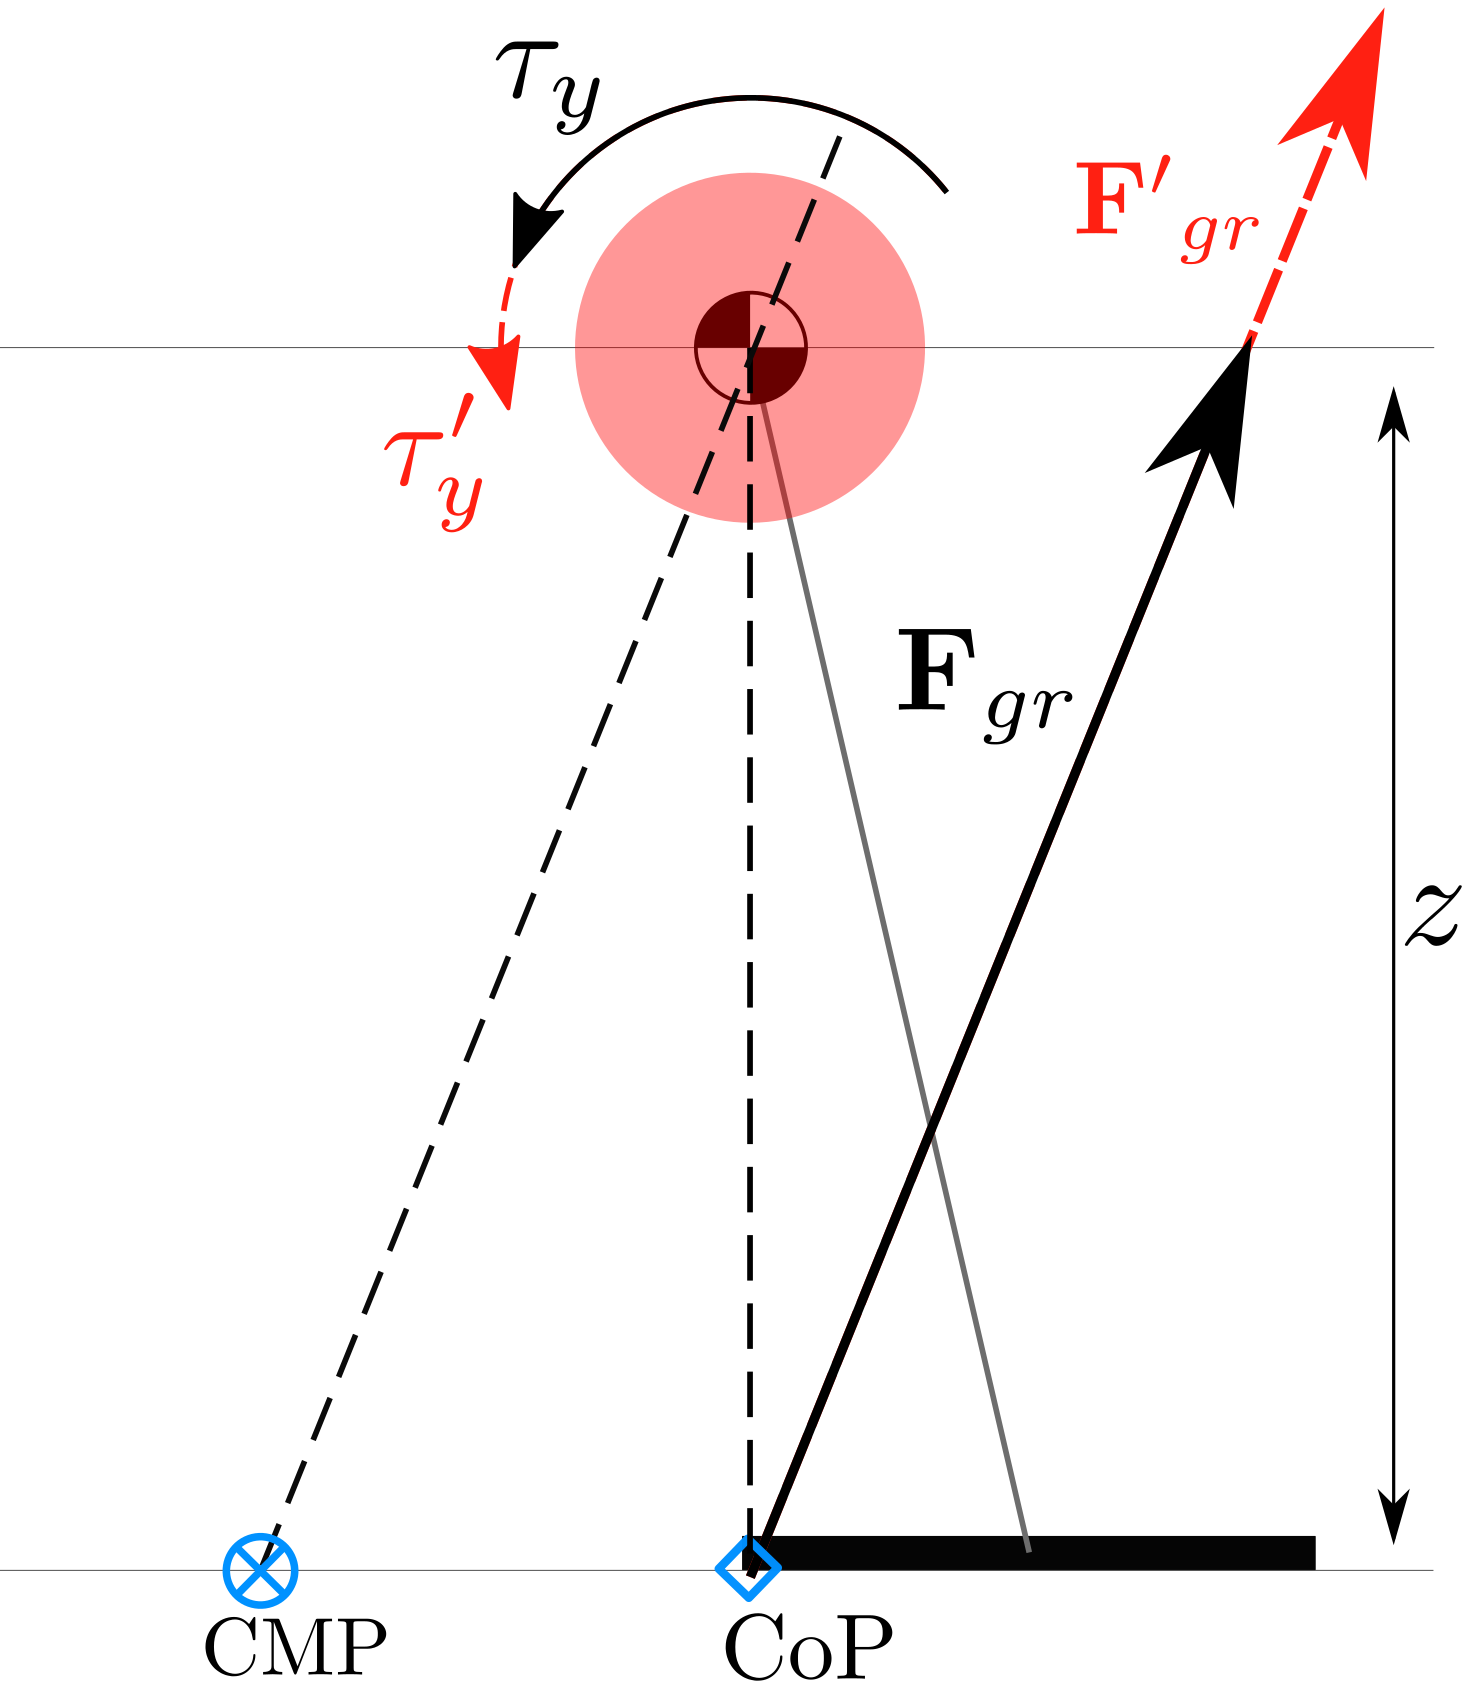
\includegraphics[width=.8\linewidth]{STYLESTUFF/2DCMPVIZCoPzero.png}
  \caption{}
   \label{fig:cmpFzb}
  \end{subfigure}
  \begin{subfigure}{0.35\textwidth}
    \centering
  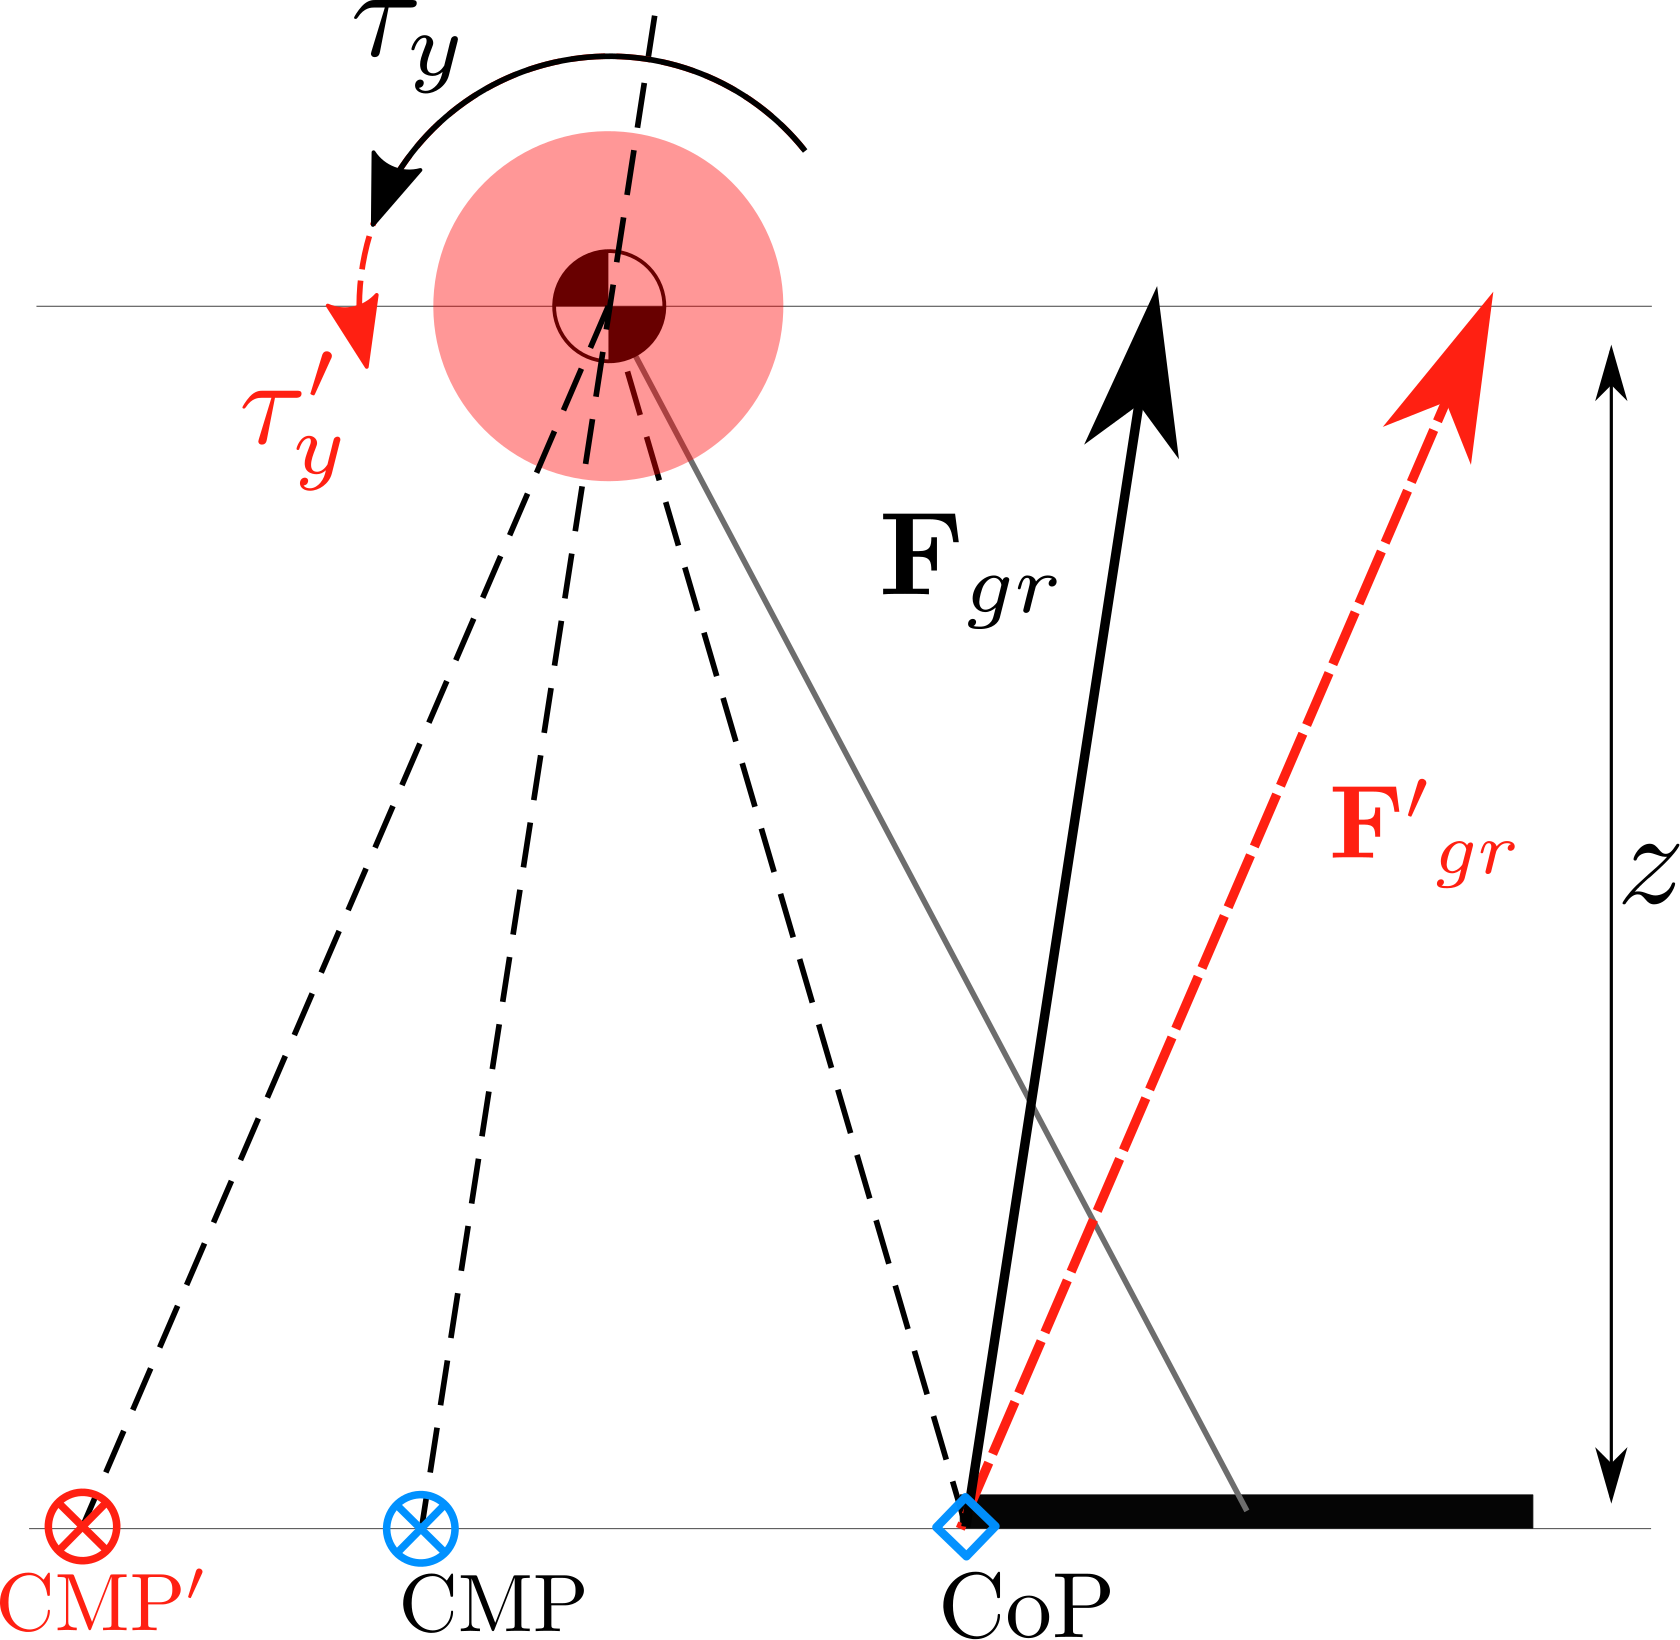
\includegraphics[width=.8\linewidth]{STYLESTUFF/2DCMPVIZFgradjusted.png}
    \caption{}
     \label{fig:cmpFzc}
  \end{subfigure}
  \caption{}
  \label{fig:cmpFz}
\end{figure}
\subsection{From 2D to 3D}
Gram determinant. Growth unstable eigenvalue. Coupling xy. 1 input for directions.
\subsection{Predictability of Dynamics}
Wether or not to recover, given foot holds, force limits, height limits, friction limits.
\subsection{Singularity Avoidance}
Stance leg and swing leg. 
% Methods
\section{Methods}
Best you can do. No MPC. Considering footholds are given. Speeding up trajectory?
\subsection{Adjust Quadratic Program Structure}
\subsection{Adjust Quadratic Program Inputs}
Harsh touchdown. Singularity of stance and swing leg. Different strategies. 

\begin{equation}
\dot{\mathbf{l}}_d=\frac{\mathbf{c}_{xy}-\mathbf{r}_{cmp,d}}{z}F_z
\end{equation}

\begin{equation}
\dot{\mathbf{l}}_d=\frac{\mathbf{c}_{xy}-(\mathbf{r}_{cop,d}+\frac{\tau_y}{F_z})}{z}F_z
\end{equation}

\begin{equation}
\dot{\mathbf{l}}_d=\frac{\mathbf{c}_{xy}-\mathbf{r}_{cop,d}}{z}m(g+\ddot{z}_d) - \frac{\tau_y}{z}
\end{equation}
 
 \begin{equation}
\dot{\mathbf{l}}_d=\underbrace{ \frac{\mathbf{c}_{xy}-\mathbf{r}_{cmp,d}} {z}mg}_{\dot{\mathbf{l}}_{d,lip}}  + \underbrace{\frac{\mathbf{c}_{xy}-\mathbf{r}_{cop,d}}{z}m\ddot{z}_d}_{\dot{\mathbf{l}}_{d,heightcontrol}}
\end{equation}
% Experimental Setup
\section{Experimental Setup}
Terrain with limited foot placement options. Push recovery

% Results
\section{Results}
\subsection{Simulation}
Comparison with `normal' control setup. (Comparison with cop / angular momentum?)
\subsection{Hardware}

% Discussion
\section{Discussion}
